\documentclass[conference]{IEEEtran}
\IEEEoverridecommandlockouts
\usepackage{cite}
\usepackage{amsmath,amssymb}
\usepackage{algorithmic}
\usepackage{algorithm}
\usepackage{graphicx}
\usepackage{booktabs}
\usepackage{url}
\usepackage{xcolor}
\graphicspath{{figs/}}
% [TODO] / [VERIFY] markers render in red so none survive unnoticed
\newcommand{\todo}[1]{\textcolor{red}{[TODO: #1]}}

\begin{document}
\title{Bounded Queues Before Learned Placement: Autonomous Management of a
UAV-Borne 5G Cell for Search-and-Rescue Robots}

\author{
\IEEEauthorblockN{Innocent Makhubela}
\IEEEauthorblockA{\textit{Department of Electrical Engineering}\\
\textit{University of Cape Town}\\
Cape Town, South Africa\\
mkhinn011@myuct.ac.za}
\and
\IEEEauthorblockN{Joyce Mwangama}
\IEEEauthorblockA{\textit{Department of Electrical Engineering}\\
\textit{University of Cape Town}\\
Cape Town, South Africa\\
joyce.mwangama@uct.ac.za}
}
% [TODO] author list and order to be confirmed by the author

\maketitle
% Abstract (<= 250 words; count with: detex sections/abstract.tex | wc -w)
\begin{abstract}
Autonomous management of a 5G cell carried by an unmanned aerial vehicle (UAV)
must keep search-and-rescue robots commandable without an operator and without
knowing the terrain. Over an OpenAirInterface and Open5GS testbed serving four
robots, we built and flew a three-loop management stack: a per-robot uplink cap
(every 0.2\,s), a liveness monitor (every 20\,s), and a terrain-blind learning
layer that forecasts link failure and places the UAV in three dimensions (every
30\,s). The decisive loop was the simplest. Long forest outages were not
coverage loss but uplink queuing inside the user equipment (UE): constant-rate
video exceeded what the links drained and held command-and-control (C2) traffic
minutes behind it. The cap, driven only by round-trip time and bytes sent,
raised forest C2 availability from 66.8\,\% to 91.8\,\% in a patrol test and
cut the median C2 outage from 143\,s to 17\,s in a placement run. A second
silent failure, dead UE processes, had contaminated 12.4\,\% of the training
data. With both handled, the learning layer forecasts C2 failure 20\,s ahead
with modest skill that falls as model capacity grows, and neither a linear nor
a gradient-boosted model recovers how terrain changes the effect of altitude.
Over repeated missions with the cap, no learned placement beat fixed hover:
in open field every arm was within 5 points of it, and in forest the arms that
moved the UAV trailed it. For autonomous management
of such cells, sound inner loops, with bounded queues and verified liveness,
must come before learned placement.
\end{abstract}

% Introduction. Claims: paper/CLAIMS.md; novelty: paper/NOVELTY.md
\section{Introduction}
\label{sec:intro}

After an earthquake, flood or fire, the ground robots sent to search a
disaster site need a mission-critical link for command and control (C2) and
video, and the terrestrial network they would use is often gone or
overloaded~\cite{murphy2014disaster}. A 5G base station (gNB) carried by an
unmanned aerial vehicle (UAV) can bring a private cell to the
robots~\cite{zeng2016wireless,mozaffari2019tutorial}. Such a cell has to be
managed: something must decide where to fly it, notice when a robot is about
to lose its link, and keep the links usable under the load the robots put on
them. On site there is no operator to tune it and no reliable map of terrain
that may have just changed, so the management has to be autonomous, proactive
and blind to the terrain, which is the setting of zero-touch
management~\cite{coronado2022zsm}.

Our earlier testbed study~\cite{makhubela2026satnac} showed that terrain decides
whether moving such a node helps: an uninformed roaming node raised a weak
robot's C2 availability in open field and cost about 22 points in forest. The
natural next step is a learning-based management layer that forecasts link
failures and places the UAV in three dimensions without being told the terrain.
This paper builds that layer as part of a three-loop management stack
(Fig.~\ref{fig:arch}), flies it in closed loop over real 5G software, and asks
what each loop delivers. The answer turned out to depend less on the learning
than on whether the managed system was measured and loaded soundly.

We test four claims, each against an explicit control (Section~\ref{sec:setup}):
\begin{itemize}
\item[\textbf{C1}] Long forest outages under robot video are caused by uplink
queuing inside the user equipment (UE), not by coverage, and a delay-adaptive
uplink cap at each robot removes them without starving strong links.
\item[\textbf{C2}] A terrain-blind model forecasts the onset of C2 failure
20\,s ahead on an unseen terrain better than chance, and higher-capacity models
do worse.
\item[\textbf{C3}] Terrain-blind models do not recover how terrain changes the
effect of altitude, so they cannot choose altitude.
\item[\textbf{C4}] Learned placement does not beat fixed hover, over repeated
missions in two terrains.
\end{itemize}
C1 holds; C2 and C4 hold weakly; C3 holds as a negative result.

\textit{Contributions.} The work falls under wireless and 5G networks,
mission-critical networks, proactive and autonomic management, artificial
intelligence (AI)-based management, monitoring and measurement, and testbed
experimentation. Beyond the testbed and terrain comparison
of~\cite{makhubela2026satnac} (Table~\ref{tab:satnac}), it contributes:
\begin{enumerate}
\item \emph{A diagnosis and an autonomic fix.} The forest outages are a silent
queueing failure of the managed system. A per-robot cap driven only by
round-trip time and bytes sent, with no change to the radio access network
(RAN), shortens outages from minutes to seconds and lifts both placement arms
flown with and without it (Section~\ref{sec:r-cap}).
\item \emph{A liveness monitor with a measurement-integrity check.} A second
silent failure, the UE process dying after radio-link failure, contaminated
12.4\,\% of training observations; we give a mechanistic detection rule and
validate it against the monitor's own record (Section~\ref{sec:dead}).
\item \emph{An evaluation of terrain-blind learning for proactive management}
on held-out terrain and in closed loop, with the negative results stated
(Sections~\ref{sec:r-forecast} and~\ref{sec:r-flip}).
\item \emph{A closed-loop account of learned placement}, showing why a single
mission is too short to learn the forest's altitude effect and why a cautious
learner reduces to hover (Section~\ref{sec:r-place}).
\end{enumerate}
All results come from emulation over real 5G software; a hardware trial is the
next step.

% Related work (0.5 p). Refs: SATNAC list (author-supplied) + web-verified (refs.bib verify_note)
\section{Background and Related Work}
\label{sec:related}

\textit{Aerial base stations and their testbeds.} The elevation-dependent
line-of-sight model~\cite{alhourani2014modeling} underlies most work on where
to place a UAV base station, from 3-D placement~\cite{boryaliniz2016efficient,
kalantari2016number} and trajectory design~\cite{wu2018common} to deep
reinforcement learning~\cite{qiu2020placement}; surveys cover the wider
field~\cite{zeng2016wireless,mozaffari2019tutorial}. These works optimise
coverage or rate under an analytic or simulated channel. Testbeds now run
OpenAirInterface on UAVs with O-RAN control~\cite{moore2024aerpaw} or emulate
5G mobility with ray tracing~\cite{iye2025owdt}. Our earlier
study~\cite{makhubela2026satnac} coupled a real 5G stack to a terrain
simulator and found that terrain decides whether moving the node helps.

\textit{Learning-based and autonomous management.} Zero-touch management aims
at fully autonomous operation under human oversight~\cite{coronado2022zsm}, and
O-RAN exposes closed control loops at sub-second to minute time scales in which
learned controllers can run~\cite{polese2023oran}; our three loops sit at the
same three scales, but outside the RAN.
Machine learning for link-quality estimation~\cite{cerar2021lqe}, fault
management~\cite{mulvey2019fault} and failure prediction in 5G RANs, with deep
and transformer models~\cite{islam2023dnn,hasan2024gentrap}, learns from the
history of a deployed network. A UAV arriving at a disaster site has no such
history for its terrain, so we test on an unseen terrain and in closed loop.

\textit{Buffering in cellular links.} Buffers that hold rather than drop
packets inflate delay~\cite{gettys2012bufferbloat}, and per-user cellular
buffers are a known source~\cite{jiang2012tackling}. Remedies range from active
queue management~\cite{nichols2012codel} and delay-aware rate
control~\cite{winstein2013sprout} to, recently, RAN-side congestion marking:
in 5G, time spent in the radio link control (RLC) buffer dominates one-way
delay~\cite{wan2025l4span}, retransmission and uplink-scheduling buffers can
add delay comparable to congestion~\cite{liu2025fog}, and sizing the RLC buffer
dynamically cuts that delay~\cite{irazabal2022buffer}. Those remedies change
network queues, the RAN or the transport protocol. Our cap applies the classic additive-increase,
multiplicative-decrease (AIMD) rule~\cite{chiu1989aimd} to a delay signal at the robot, because constant-rate
robot video does not back off and the UE's buffer is not ours to change.

% Draft table: what is new over SATNAC 2026 (sources: published SATNAC text,
% pasted by the author 2026-11-12; this paper's Sections III-V).
\begin{table}[t]
\caption{This Paper Versus Our Earlier Study~\cite{makhubela2026satnac}}
\label{tab:satnac}
\centering\footnotesize\setlength{\tabcolsep}{3pt}
\begin{tabular}{@{}p{0.2\columnwidth}p{0.36\columnwidth}p{0.38\columnwidth}@{}}
\toprule
 & SATNAC 2026 & This paper \\
\midrule
Robots & 2 & 4 \\
UAV control & fixed hover vs.\ random walk & forecaster, planner, altitude learners vs.\ hover and centroid \\
Management loops & rule-based coverage guard & uplink cap, liveness monitor, learned x--y--z placement \\
Traffic & 2-s 8\,Mb/s bursts per cycle & continuous 1.5\,Mb/s video per robot \\
C2 available & $\geq$1 of 5 echoes answered & ping loss $<$\,50\,\% \\
Validation & static vs.\ roaming phase, one run per terrain & held-out terrain, null controls, repeated seeds \\
Main finding & mobility helps in open field, hurts in forest & bound queues and check liveness first; learning ties simple rules \\
\bottomrule
\end{tabular}
\end{table}


% System and method. Sources: docs/SYSTEM_ARCHITECTURE.md, scripts/ml/{onset_forecast,
% planner,online_planner,altitude_bandit,geo_features}.py, scripts/adaptive_uplink_cap.py
\section{System and Method}
\label{sec:method}

The management stack has three loops at three time scales
(Fig.~\ref{fig:arch}): a per-robot uplink cap that reacts within a second
(Section~\ref{sec:cap}), a liveness monitor that checks every 20\,s that each
UE process is alive (Section~\ref{sec:dead}), and a terrain-blind learning
layer that decides every 30\,s where the UAV goes (Section~\ref{sec:layer}).
The inner loops keep the managed system sound; the outer loop optimises it.

\subsection{Platform}
\label{sec:platform}
The managed system is the protocol-in-the-loop testbed
of~\cite{makhubela2026satnac}, extended from two to four robots
(Fig.~\ref{fig:arch}). An OpenAirInterface (OAI)~\cite{nikaein2014oai} gNB and
four OAI UEs run over the OAI radio simulator and register to an
Open5GS~\cite{open5gs} core (OAI commit 09c9bb998f). The cell uses band n78 at
3.32\,GHz with 106 resource blocks at 30\,kHz spacing (40\,MHz) and a 5-ms
time-division pattern of five downlink and four uplink slots; every simulated
channel is additive white Gaussian noise (AWGN), so there is no multipath. Each UE's virtual network (TUN) interface sits in its own Linux
network namespace, so robot traffic crosses the real 5G user plane. Gazebo
moves the UAV and four ground robots; a bridge reads their poses every 0.5\,s
and writes a terrain-specific air-to-ground path loss into each UE's channel:
free-space loss with an elevation-dependent line-of-sight
term~\cite{alhourani2014modeling}, plus foliage~\cite{weissberger1982},
diffraction~\cite{itup526} or building loss by terrain, and correlated
shadowing~\cite{gudmundson1991} (details in~\cite{makhubela2026satnac}). A
watchdog relaunches a UE whose process exits after radio-link failure.

\begin{figure*}[t]
\centering
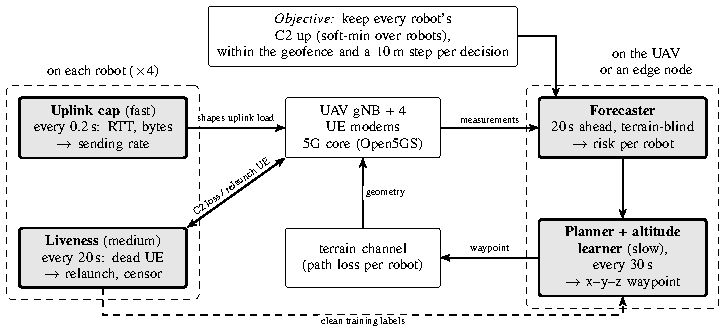
\includegraphics[width=0.82\textwidth]{fig_arch.pdf}
\caption{Management architecture, deployment view: three loops at three time
scales around the managed cell. The cap and the liveness monitor would run on
each robot, the learning layer on the UAV or an edge node; in the testbed all
run on one host. The liveness monitor also cleans the labels the learning layer
is trained on.}
\label{fig:arch}
\end{figure*}

\subsection{Liveness Monitor and Measurement Integrity}
\label{sec:dead}
In OAI, a radio-link failure terminates the UE process, after which the
robot's C2 stays down whatever the UAV does. The liveness monitor probes each
robot's C2 every 20\,s. After 90\,s of total C2 loss it checks the uplink from
inside the robot's namespace and, if the UE is gone, relaunches that UE alone,
giving up after three failed attempts.

The same failure contaminates data recorded before the monitor worked. Once a
UE process dies, the gNB's per-UE counters freeze, and the cycles are logged as
link failures although they record a dead process; a model with lagged
features spots them trivially (the change in block error rate is exactly zero).
We flag a cycle as dead when, for at least three consecutive cycles, the gNB
counters \texttt{dl\_bler}, \texttt{ul\_nb\_rbs} and \texttt{ul\_bits\_per\_sym}
are bit-identical to the previous cycle \emph{and} C2 is down. Frozen counters
on a working link are a quiet cycle, and a failed cycle with moving counters is
a real degradation, so both conditions are required. The rule flags 12.4\,\%
of all cycles and 72.2\,\% of hills failure labels (Table~\ref{tab:a1}), and
flagged cycles are censored. Checked against the monitor's own record of dead or
relaunching UEs, in the 29 of 80 robot series where the monitor was running,
85\,\% of the rule's flags agree, but the rule finds only 56\,\% of the dead
cycles the monitor saw, so some contamination remains in the older data.
% A4: dead_process_extent.csv; rule: onset_forecast.py dead_ue_mask (FREEZE_MIN);
% validation: logs/ml/dead_process_validation.csv; monitor constants: auto_patrol.py RLF_CONFIRM_S, WATCHDOG_PERIOD_S, RLF_MAX_FAILURES

\subsection{Terrain-Blind Learning Layer}
\label{sec:layer}
\textit{Forecaster.} The label is the onset of C2 failure: for a robot whose C2
is up at time $t$, is it down at $t+20$\,s? C2 is up when fewer than 50\,\% of
its probes are lost. Features are UAV--robot geometry, gNB-side link
adaptation and error statistics, and the last commanded move, each with lags,
differences and rolling statistics within one robot's series (65 features).
Three inputs are forbidden: the simulator's injected path loss, the computed
received power (algebraically equivalent to it), and any terrain label. A guard
function checks every feature matrix before it reaches an estimator. Models are
trained leave-one-terrain-out, with thresholds and calibration chosen on an
inner time split of the training terrains.

\textit{Planner.} Each 30-s decision, the planner scores candidate UAV
positions (absolute altitudes 25--55\,m in 5\,m steps, crossed with lateral
offsets of 0 or 15\,m) by a soft minimum over the robots' predicted risks,
$J(u) = \beta^{-1}\log\sum_i e^{\beta r_i(u)}$ with $\beta = 10$, so the
worst-served robot dominates. It moves toward the minimiser at most 10\,m in
altitude per decision. The planner's risk model is the same logistic
regression with spline terms on altitude, distances and elevation angle and
Platt calibration (pooled held-out area under the receiver operating
characteristic curve, ROC-AUC, 0.659). In every fly-off the
planner uses the model trained on the other three terrains, never on the
terrain it flies over.

\textit{Altitude learner.} Because the model cannot choose altitude
(Section~\ref{sec:r-flip}), altitude is learned during the mission. The learner
holds an incumbent altitude and rewards each altitude by the fraction of robots
with C2 up. Its estimates are time-blocked (240\,s blocks), so only comparisons
made close in time count. Every few decisions it probes a neighbouring altitude
($\pm$5 or 10\,m), and it moves when the lower confidence bound of the
neighbour-minus-incumbent difference is above zero ($z = 0.5$). The
\emph{cautious} variant adds a home altitude, the hover altitude of 40\,m: a
move further from home must clear 1.5 standard errors \emph{and} a 0.02 gain,
a move back toward home only the normal bar, and probes are rarer (every 4th
decision, every 20th once all neighbours are worse).
% planner.py (Z_TARGETS, DXY_R, MAX_DZ_STEP, beta=10); altitude_bandit.py AltitudeProber; online_planner.py CAUTIOUS

\subsection{Delay-Adaptive Uplink Cap}
\label{sec:cap}
The cap moves the bottleneck from the UE into the robot's kernel, where it can
be bounded and prioritised, and lets its rate follow the link. It needs no
change to the RAN or core. On each robot's TUN interface, a hierarchical token bucket (HTB) shaper has a
ceiling equal to the cap $c$. C2 and ping (ICMP) traffic use a high-priority class with a
20-packet queue; video uses a low-priority class with a 10-packet queue, so
excess video is dropped rather than buffered. Each robot pings the core every
0.2\,s. ICMP bypasses the kernel video queue, so its round-trip time (RTT) rises only when the
UE's own buffer backs up. With $r_0$ the minimum RTT over 60\,s and $\tilde r$
the median over the last second, Algorithm~\ref{alg:cap} runs every 0.2\,s.
The ``in use'' test keeps an idle robot's cap from rising and then overloading
the link when video resumes. The controller re-creates the shaper when a UE
reattaches with a new TUN. Its only inputs, RTT and bytes sent, are available
on real hardware.

\begin{algorithm}[t]
\caption{Per-Robot Uplink Cap (Every 0.2\,s)}
\label{alg:cap}
\begin{algorithmic}[1]
\small
\STATE initially $c \leftarrow 200$\,kb/s, $\mathit{slow} \leftarrow$ true
\IF{$\tilde r > r_0 + 150$\,ms \OR no reply for 1\,s}
  \STATE $c \leftarrow \max(50,\,0.7c)$; $\mathit{slow} \leftarrow$ false; hold 2\,s
\ELSIF{$\tilde r < r_0 + 50$\,ms \AND sent $\ge 0.7c$ \AND 2\,s since last raise}
  \STATE $c \leftarrow \min(1600,\ \mathit{slow}\ ?\ 2c : c + 50)$
\ENDIF
\end{algorithmic}
\end{algorithm}
% adaptive_uplink_cap.py constants: LO,HI,START=50,1600,200; CUT .7; STEP 50; HOLD 2; UP_EVERY 2; HIGH 150; LOW 50; BASE_WIN 60

% Experimental setup. Sources: EVIDENCE.md A-E, run_*_flyoff.sh, video_streams.py
\section{Experimental Setup}
\label{sec:setup}

\textit{Traffic and metrics.} Each robot sends constant-rate UDP (User Datagram Protocol) video at
1.5\,Mb/s to the core and is probed for C2 by ping; a robot's C2 is up when
fewer than 50\,\% of its probes are lost. These definitions differ from those
of~\cite{makhubela2026satnac} (two robots, 8\,Mb/s video bursts, C2 up when
any of five echoes returns), so numbers are not comparable across the two
papers. Placement runs are reported as the time-weighted share of a mission
with mean C2 up, with all four robots up, and with no robot up, and the
90th-percentile video latency. Forecasts are scored by the area under the
precision--recall curve (PR-AUC) relative to the no-skill rate (lift) and by ROC-AUC, pooled over held-out terrains and on the
worst held-out terrain.

\textit{Data.} The forecasting and altitude-effect results use 54,572
robot-cycles from 20 missions of 90--200\,min over four terrains (open field,
urban, forest, hills), all flown before the cap existed. The cap was tested in
a static load test in forest and open field (6\,min of video between 2-min
no-load phases), in a 30-min forest patrol, and in the placement fly-offs.

\textit{Placement arms.} Every arm flies the same pilot, seed and 90-min
mission and differs only in how x--y and altitude are chosen
(Table~\ref{tab:arms}): the pilot decides every 30\,s, changes altitude by at
most 10\,m per decision, and stays within a 20--60\,m geofence. The 40-m hover altitude and the
20--60\,m band are those of~\cite{makhubela2026satnac}: 40\,m is the middle of
the band and clears every obstacle in the outdoor worlds. Arm B, the
robot centroid at fixed altitude, is the baseline of our research proposal; arm
A, fixed hover, is the simplest policy; the repositioning policy
of~\cite{makhubela2026satnac} is a further baseline for the risk planner.

\begin{table}[t]
\caption{Placement Arms}
\label{tab:arms}
\centering
\small
% Table 1 (hand-written: definitions, no numbers). Source: run_xyz_flyoff.sh,
% scripts/ml/online_planner.py (SAR_PLANNER_XY / _ALT / _ALT_LEARNER).
\begin{tabular}{@{}llll@{}}
\toprule
Arm & x--y & Altitude & Role \\
\midrule
A & held & fixed 40\,m & baseline (hover) \\
B & robot centroid & fixed 40\,m & baseline (proposal) \\
C & robot centroid & learned on the spot & learned altitude \\
D & risk model & learned on the spot & learned x--y--z \\
\bottomrule
\end{tabular}

\end{table}

\textit{Validation protocol.} A result is accepted only after it survives the
control that matches its threat: leave-one-terrain-out evaluation with
worst-fold reporting for forecasting; censoring of dead-process cycles for every
label; a same-policy null control (the same comparison applied to two nights of
one policy) for closed-loop comparisons made across nights, where a
comparison counts only if the null control's interval rules out a swing as
large as the effect; and the uplink cap
for any forest outcome. Confidence intervals are 95\,\% block bootstraps over
contiguous stretches (10-min blocks for missions), because consecutive cycles
are strongly correlated; an effect whose interval includes zero is reported as
not established. Per-arm placement comparisons use one 90-min run per arm and
within-run intervals, which do not capture run-to-run variation.
\todo{update: three seeds per arm in forest and open field from the repeat campaign}

% Results. Every number: see paper/figs/README.md and paper/EVIDENCE.md (IDs in comments).
\section{Results}
\label{sec:results}

\subsection{C1: Uplink Queuing, Not Coverage, and an Autonomic Cap}
\label{sec:r-cap}

\textit{The long forest outages are a queue inside the UE.} With the four
robots parked under canopy (24--30\,dB uplink attenuation) and the UAV at
40\,m, C2 was clean without load. Once the four 1.5\,Mb/s video feeds started,
uplink ping RTT grew from about 60\,ms to minutes within the first seconds and
kept rising for the whole load period, peaking at 350--444\,s
(Fig.~\ref{fig:rtt}(a)); 64--91\,\% of pings were lost and, for 64\,\% of the
time, all eight probes (one per direction per robot) were lost at once (Table~\ref{tab:static}). Probes were
delayed rather than dropped, and the links drained only 0.13--0.49\,Mb/s of the
1.5\,Mb/s offered. The kernel queue on each robot's TUN interface held no backlog and dropped
nothing, so the excess was buffered beyond the kernel, inside the OAI UE
software (E1); we did not instrument which UE layer holds it. The drain rate is
not simply what the radio supports: in the capped placement runs the gNB's own
counters (modulation, code rate, allocated symbols) implied full-carrier uplink
rates of tens of Mb/s even in forest, far above 1.5\,Mb/s, and the emulator's
radio thread ran near one full core. Whether the limit is scheduling or
emulation is under measurement.
\todo{capacity sweep 0--35\,dB and 1/2/4-robot saturation, with gNB MAC
statistics and per-thread CPU (scheduled 15 Nov)} After the video stopped, C2 stayed dead for 14 to more than 18\,min,
consistent with each link slowly draining its backlog.

% E1: tab_static_load (analyse.py), ul_*.txt max RTT, CONGESTION_TEST_REPORT.md (qdisc); 79 MB figure removed (untraceable, review K6)
\begin{figure*}[t]
\centering
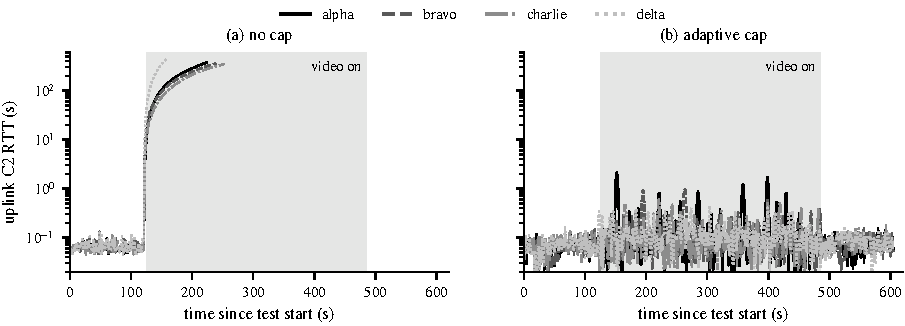
\includegraphics[width=\textwidth]{fig_rtt.pdf}
\caption{Uplink C2 ping RTT per robot in the static forest load test (log
scale; video on in the shaded interval). (a) Without a cap, RTT grows to
minutes; traces end where replies stop before the test ends. (b) With the
adaptive cap, RTT stays near its unloaded level.}
\label{fig:rtt}
\end{figure*}

\begin{table}[t]
\caption{Static Forest Load Test, Four Robots, 6\,min of Video}
\label{tab:static}
\centering
\footnotesize\setlength{\tabcolsep}{3pt}
% generated by tab_static_load.py -- do not edit
\begin{tabular}{@{}lccc@{}}
\toprule
 & No cap & Fixed 100\,kb/s & Adaptive \\
\midrule
Uplink ping loss, video on & 64--91\,\% & 0\,\% & 0\,\% \\
Uplink ping RTT, median & 3--4\,min & 69--87\,ms & 76--108\,ms \\
All probes lost (on / off) & 64 / 100\,\% & 0 / 0\,\% & 0 / 0\,\% \\
Recovery after video & 14--18+\,min & none & none \\
Video goodput (Mb/s) & 0.13--0.49 & 0.10 & 0.10--0.42 \\
Video latency, median & 2.2--2.8\,min & 1.08--1.11\,s & 0.30--1.08\,s \\
\bottomrule
\end{tabular}

\end{table}

\textit{Bounding the queue removes the outages.} A fixed 100\,kb/s cap below
every link's drain rate, applied at the same placement, removed all C2 loss and
the recovery tail, but discarded most of the video (Table~\ref{tab:static}).
The adaptive cap of Section~\ref{sec:cap} also gave zero C2 loss while settling
at a different rate on each link (medians 105--429\,kb/s, 32--40 cuts per robot
in 6\,min), delivering 0.10--0.42\,Mb/s of video at a median latency of
0.30--0.42\,s on three robots; the fourth, with the weakest link, ran at
1.08\,s, the time its 10-packet video queue takes to drain at about 100\,kb/s
(Fig.~\ref{fig:rtt}(b)). In open field, with 2--9\,dB of attenuation, every cap
rose to its 1.6\,Mb/s ceiling, made no cuts, and carried the full 1.55\,Mb/s
per robot at 82--89\,ms median latency (E4): in this test, where links were
strong, the cap stayed out of the way.
% E2, E3: cap_log.csv (medians, cuts), tab_static_load; E4: CONGESTION_TEST_REPORT follow-up 3

\textit{The cap lifts the like-for-like placement arms.} In a 30-min forest patrol with
the UAV hovering at 40\,m, the cap raised mean C2 availability from 66.8\,\% to
91.8\,\% against the same seed uncapped, cut the time with no robot connected
from 17.4\,\% to 0.9\,\%, and the 90th-percentile video latency from 73\,s to
1.6\,s (Table~\ref{tab:a5}). In the forest fly-off (Fig.~\ref{fig:caparms}), only arms A and B flew
the same policy with and without the cap: there, the time with no robot
connected fell from 25.4 and 25.9\,\% to 0.3 and 0.0\,\%, and mean C2 rose from
66.6 and 58.0\,\% to 89.1 and 88.9\,\%. Arms C and D also changed altitude
learner between the two conditions, so their improvement cannot be attributed
to the cap alone. Each comparison is one run per condition on different
nights, with no null control for those nights.

\textit{The cap turns minute-long outages into single missed cycles.} For the
same like-for-like runs, Fig.~\ref{fig:outage} gives the length of every C2
outage. Without the cap the median forest outage lasted 143\,s (arm A) and
97\,s (arm B), and 64\,\% and 59\,\% of outages exceeded a minute; with it
the medians fell to 17\,s and 19\,s and 11\,\% and 19\,\% exceeded a minute.
In open field the median fell from 48\,s to 11\,s (Table~\ref{tab:a6}).
Capped forest runs had somewhat more outages per robot-hour (12.2 against 7.0
for arm A), almost all a single measurement cycle long; at 11--20\,s per cycle,
that is the shortest outage the logs can resolve.

\begin{figure}[t]
\centering
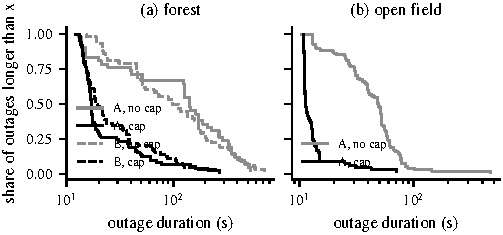
\includegraphics[width=\columnwidth]{fig_outage.pdf}
\caption{Length of C2 outages (time a robot's C2 stayed down), like-for-like
arms with and without the cap, one 90-min run each: share of outages longer
than a given duration. Durations below about 15\,s are not resolved.}
\label{fig:outage}
\end{figure}

The same mechanism may bear on the forest result of our earlier
study~\cite{makhubela2026satnac}, where a roaming node drove 8\,Mb/s video
bursts to over 70\,\% loss; its traffic pattern differed, and we have not
tested this.

\textit{Cap versus 5G-native separation.} A separate network slice or QoS flow
for C2 would also keep C2 out of the video queue, but not shorten the video's
own delay. \todo{slice-per-traffic-class experiment: no cap, cap, slice, slice
+ cap, static forest load test and one patrol}
% E5: tab_a5_patrol; E6: fig_cap_arms (summary CSV, sets xyz/capped)

\begin{figure}[t]
\centering
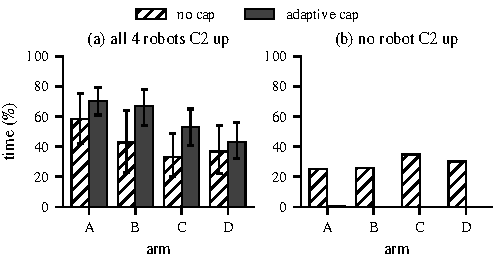
\includegraphics[width=\columnwidth]{fig_cap_arms.pdf}
\caption{Forest fly-off, each placement arm without and with the adaptive cap
(one 90-min run per bar; whiskers: 95\,\% block-bootstrap CI). Arms C and D
used an upper-confidence-bound (UCB) altitude bandit uncapped and the prober
learner capped, so only A and B flew the same policy in both conditions.}
\label{fig:caparms}
\end{figure}


\subsection{C2: Terrain-Blind Forecasting Has Modest Skill, and Capacity Hurts}
\label{sec:r-forecast}

\textit{A linear model forecasts failure onset 20\,s ahead on unseen terrain,
weakly.} After dead-process censoring (Section~\ref{sec:dead}), the best
model, an L1-regularised logistic regression on 65 terrain-blind features,
reaches a pooled PR-AUC 1.79 times the no-skill rate and ROC-AUC 0.667, and no
held-out terrain falls below ROC-AUC 0.538 (Fig.~\ref{fig:capacity}). Skill
peaks at a 20-s horizon: a six-feature trend model scores ROC-AUC 0.650 at
20\,s and 0.552 at 60\,s (Table~\ref{tab:a2}). Forest labels in this data
predate the cap and are partly queue backlog (Section~\ref{sec:r-cap}).
\todo{retrain all eight model classes on the capped, monitor-protected runs and
report beside these numbers}
% A6: phase2c_model_class.csv; A5: phase2b_onset.csv

\begin{figure}[t]
\centering
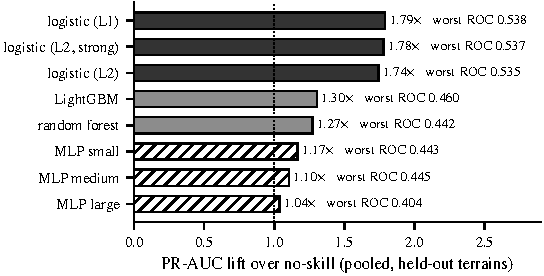
\includegraphics[width=\columnwidth]{fig_capacity.pdf}
\caption{Forecasting skill by model class: pooled PR-AUC lift over no skill
on held-out terrains, and the worst held-out-terrain ROC-AUC (65 features,
20-s onset horizon, 38,303 onset observations, leave-one-terrain-out).}
\label{fig:capacity}
\end{figure}

\textit{More capacity is worse.} On identical folds and features the ordering
is monotone in capacity: three linear models lead, tree ensembles follow, and
three multilayer perceptrons trail. The largest network scores ROC-AUC 0.503,
and 0.404 on its worst terrain, below chance. One exception should be stated:
on six trend features at a 60-s horizon, the medium network beats the linear
models on pooled lift (1.55 against 1.21--1.22) but not on its worst terrain (ROC
0.456 against 0.550). Sequence models on 10\,Hz radio traces add nothing: on
3,115 labelled cycles over three folds, a temporal convolutional network (TCN) and a gated recurrent unit (GRU)
average ROC-AUC 0.493
and 0.523 against 0.540 for a logistic regression on window summaries (A7).
Under leave-one-terrain-out validation with four terrains, we take worst-fold
skill, not pooled skill, as the figure of merit; our reading is that it rewards
models that learn a direction rather than thresholds tied to the training
terrains.
% A6 exception: phase2c n==38803 block, trend6 mlp_medium 1.551 / worst 0.456 vs logistic_L2 1.221 / 0.551; A7: phase6_seq.csv

\subsection{C3: The Model Does Not Recover How Terrain Changes the Altitude Effect}
\label{sec:r-flip}

The measured effect of climbing differs strongly between terrains: per +10\,m,
C2 availability gains 0.208 more in open field than in forest per cycle, and
0.167 more on a uniform 60-s time base that removes the outcome-dependent cycle
length (Table~\ref{tab:contrasts}). This terrain dependence was reported
in~\cite{makhubela2026satnac}; the question here is whether a terrain-blind
model recovers it. To give the model every chance we use a gradient-boosted
tree model (LightGBM), which can represent interactions between altitude and
link state, trained on the same terrain-blind features and held-out terrains.
It does not recover it. At the 20-s horizon of Section~\ref{sec:r-forecast}, the
open-field-minus-forest contrast in the model's risk is $+0.001$ ($p = 0.89$),
and no contrast is significant. At a 60-s horizon it is $+0.006$ ($p = 0.37$),
and two other contrasts are significantly inverted. On coarser 120-s bins one
recovered contrast reaches significance but stays about one sixth of the
measured value (Appendix~\ref{app:tables}).
% C3: tab_contrasts (phase4b_interactions measured/raw h60; phase4b_h20 raw; phase4c 60 s bins); 120 s: phase4d recovered_raw

\begin{table}[t]
\caption{Altitude-Effect Contrasts (C2 Availability per +10\,m): Measured,
and Recovered From a Terrain-Blind LightGBM Model at Two Forecast Horizons.
$^*$: 95\,\% Block-Bootstrap CI Excludes 0}
\label{tab:contrasts}
\centering
\small
\begin{tabular}{@{}c@{}}
{\footnotesize \hspace{16mm}measured\hspace{14mm}recovered}\\[-1pt]
% generated by tab_contrasts.py -- do not edit
\begin{tabular}{@{}lcccc@{}}
\toprule
Contrast & Cycle & 60-s bins & $h{=}20$\,s & $h{=}60$\,s \\
\midrule
Open $-$ forest & $+0.208$$^*$ & $+0.167$$^*$ & $+0.001$ & $+0.006$ \\
Open $-$ hills & $+0.153$$^*$ & $+0.138$$^*$ & $-0.003$ & $+0.037$$^*$ \\
Urban $-$ forest & $+0.073$$^*$ & $+0.070$$^*$ & $+0.006$ & $-0.020$$^*$ \\
Hills $-$ forest & $+0.055$$^*$ & $+0.030$ & $+0.003$ & $-0.031$$^*$ \\
\bottomrule
\end{tabular}
% measured: per cycle and 60-s uniform bins; recovered (LightGBM): per cycle at horizons 20 s and 60 s

\end{tabular}
\end{table}

The consequence for control is direct. Replayed through the planner on each
held-out terrain, no surrogate chooses altitude sensibly: linear models choose
about 55\,m in every terrain, and a gradient-boosted model chooses about 47\,m in both
forest and open field (D1). Altitude therefore has to be learned during the
mission.
% D1: logs/ml/altsel_run.log

\subsection{C4: Learned Placement Under the Cap}
\label{sec:r-place}

\textit{An exploring altitude learner did worse than the baselines in single runs.} With the cap on,
hover (A) and centroid (B) kept all four robots connected 70.5\,\% and
67.0\,\% of the time in forest, indistinguishable from each other (B$-$A
$-4.0$ [$-20.4$, $+11.2$] points). The two arms with an exploring learner were
worse within their runs: C$-$A $-18.1$ [$-34.1$, $-2.6$] and D$-$A $-27.4$
[$-43.0$, $-10.7$]. These are single runs on different nights, and the
night-to-night swings of a same-policy null control reach about 20 points
(Table~\ref{tab:a3}), so the size of the loss is not established. Both
exploring arms spent much of the mission at 45--55\,m (Fig.~\ref{fig:alt}).
% D5: capped summary + CAPPED_FOREST_FLYOFF_REPORT bootstrap table

\textit{One mission cannot determine the sign of the forest altitude effect.}
Comparing arm C with arm B at matched times, with the same x--y rule and
seed, gives $-6.6$ points of C2 per +10\,m ($[-14.9, +0.9]$): probably harmful,
not established, and too small on its point estimate to explain the whole
gap above. The slope the learner itself can estimate within one 90-min
run is $+4.6$ ($[-9.1, +12.0]$) in arm C and $+5.9$ ($[-10.7, +14.9]$) in arm
D. Its interval spans both signs, so the learner moved on noise.
% D6: logs/ml/forest_altitude_effect_capped.csv

\begin{figure*}[t]
\centering
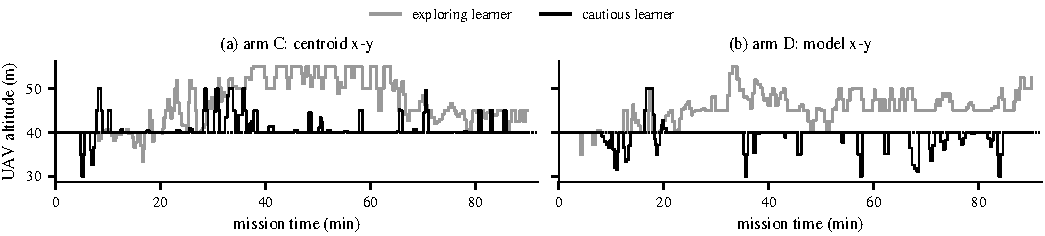
\includegraphics[width=\textwidth]{fig_altitude.pdf}
\caption{UAV altitude during the capped forest missions for the two
learned-altitude arms. The exploring learner drifts to 45--55\,m; the cautious
learner keeps 40\,m as its incumbent and leaves it only for short probes.}
\label{fig:alt}
\end{figure*}

\textit{A cautious learner behaves like hover.} Homed at 40\,m and requiring 1.5 standard
errors plus 0.02 of reward to move away, the learner kept 40\,m as its
incumbent in both arms and spent 83--84\,\% of each mission there. All four
robots were connected 65.2\,\% (C) and 72.0\,\% (D) of the time, not
distinguishable from the baselines, though the intervals are wide (C$-$A
$-5.1$ [$-17.9$, $+6.8$]; D$-$A $+1.6$ [$-13.4$, $+17.7$]),
and arm D scored $+28.8$ [$+11.9$, $+45.1$] points above its exploring version,
again a cross-night single-run comparison. In effect the cautious learner is
hover with short probes: it gave no benefit over hover. No learned arm beat a
baseline. \todo{replace with the 3-seed forest and
open-field results of the repeat campaign (Fig.~\ref{fig:seeds}); decision rule
fixed in CLAIMS.md}
% D7: cautious_forest_flyoff summary; time at 40 m: flyoff_forest_cautious_analyse.py

\begin{figure}[t]
\centering
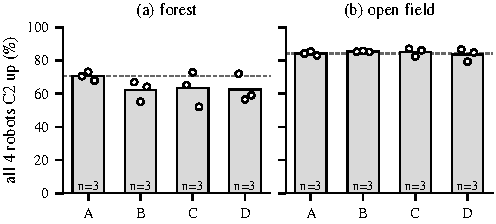
\includegraphics[width=\columnwidth]{fig_arms_seeds.pdf}
\caption{All four robots C2 up per arm with the cap, cautious learner for C
and D; bar = mean over runs, dots = individual 90-min runs. \todo{partial:
forest seed 1 only; regenerate after the repeat campaign}}
\label{fig:seeds}
\end{figure}

\textit{The risk planner survives its null control in open field only.}
Against the repositioning policy of~\cite{makhubela2026satnac}, matched on
geometry, the planner gained $+10.5$ [$+7.0$, $+13.2$] points in open field.
The same comparison between two nights of the \emph{same} baseline policy gave
$-0.5$ [$-4.3$, $+3.0$] there, which rules out a night-to-night swing of that
size, so the gain is interpretable. In forest the planner lost $-15.3$
[$-24.8$, $-5.0$], but the null control's interval [$-17.6$, $+6.4$] admits a
swing that large; in urban and hills the null was itself as large as the
effect ($+18.7$ and $-21.7$). Those three comparisons are uninterpretable
(Table~\ref{tab:a3}).
% C2: planner_vs_twophase_nullctl.csv

% Limitations (0.4 p); full version in Appendix C. Sources: docs/CHANNEL_MODEL_LIMITATIONS.md, EVIDENCE.md
\section{Limitations and Threats to Validity}
\label{sec:limits}

The radio is real 5G software, but propagation is injected: the channel has
large-scale loss and correlated shadowing but no multipath, terminal height is
fixed at 0.5\,m, and absolute availability is internally consistent rather than
externally calibrated. The OAI UE may buffer uplink data differently from a
commercial modem, and constant-rate video is a worst case for the queue;
whether C1 transfers is the first question for hardware. Every
between-terrain claim rests on four terrains. The forecasting and
altitude-effect data predate the cap, so their forest labels are partly queue
backlog, and the dead-process rule removes only about half of the dead cycles
the monitor recorded. Throughput was not measured with active probes during the
campaigns, because they would have congested the links under test; the
emulator's radio thread, near one full core, may cap the cell's total uplink
\todo{measured capacity from the 15 Nov sweep}.
Placement comparisons use one 90-min run per arm with within-run
intervals, and the robots' safety guards react to link state, so the same seed
does not give identical patrols across arms. Appendix~\ref{app:threats} gives
the full list.
\todo{revise the last-but-one sentence once the three-seed repeats are in}

% Conclusion (0.35 p)
\section{Conclusion}
\label{sec:conclusion}

We built a three-loop management stack for a UAV-borne 5G cell serving four
search-and-rescue robots and flew it in closed loop over real 5G software. The
most effective loop was not learned: a per-robot uplink cap driven by
round-trip time removed a silent queueing failure inside the UE, shortened C2
outages from minutes to single measurement cycles, and improved both placement
arms flown with and without it (C1). The learning layer forecasts
link-failure onset 20\,s ahead with modest skill that falls as model capacity
grows (C2), does not recover how terrain changes the effect of altitude (C3),
and, in closed loop, does not beat fixed hover or the robot centroid; made
cautious, it behaves like hover (C4). For autonomous management of such
cells, the lesson is to verify that the managed system is measured and loaded
soundly, bounding its queues and checking that its processes are alive, before
learning where to fly it. The next steps are a hardware trial of the cap and
retraining the layer on capped, watchdog-protected data.

\label{endofmain}

\bibliographystyle{IEEEtran}
\bibliography{refs}

\clearpage
\appendices
% Appendix: extra tables (generated), reproducibility, full threats. Drafted after main text.
\section{Extra Tables}
\label{app:tables}

\begin{table}[h]
\caption{Dead-Process Contamination by Terrain (6,760 of 54,572 rows, 12.4\,\%)}
\label{tab:a1}
\centering\small
% generated by tab_a1_dead.py -- do not edit
\begin{tabular}{@{}lccc@{}}
\toprule
Terrain & Dead share of C2-down & C2 raw & C2 censored \\
\midrule
Hills & 72.2\,\% & 83.0\,\% & 94.6\,\% \\
Forest & 53.4\,\% & 37.9\,\% & 56.7\,\% \\
Urban & 39.0\,\% & 69.6\,\% & 79.0\,\% \\
Open field & 3.9\,\% & 78.5\,\% & 79.2\,\% \\
\bottomrule
\end{tabular}
% all terrains: 6760 of 54572 rows (12.4 %)

\end{table}

\begin{table}[h]
\caption{Forecast Horizon Sweep, Censored Onset Population, Pooled Over Held-Out Terrains}
\label{tab:a2}
\centering\small
% generated by tab_a2_horizon.py -- do not edit
\begin{tabular}{@{}lcccc@{}}
\toprule
Horizon & GBM lift & GBM ROC & Logit-6 lift & Logit-6 ROC \\
\midrule
10\,s & 1.44 & 0.569 & 1.42 & 0.575 \\
20\,s & 1.29 & 0.558 & 1.52 & 0.650 \\
30\,s & 1.19 & 0.544 & 1.38 & 0.625 \\
60\,s & 1.23 & 0.579 & 1.22 & 0.552 \\
\bottomrule
\end{tabular}
% GBM = LightGBM on 65 radio_blind features (model radio_blind|raw); Logit-6 = trend logistic

\end{table}

\begin{table}[h]
\caption{Risk Planner Versus the Repositioning Baseline of~\cite{makhubela2026satnac}, With a Same-Policy Null Control (Geometry-Matched, 95\,\% CI)}
\label{tab:a3}
\centering\footnotesize\setlength{\tabcolsep}{3pt}
% generated by tab_a3_nullctl.py -- do not edit
\begin{tabular}{@{}llll@{}}
\toprule
Terrain & Planner $-$ two\_phase (pp) & Null control (pp) & Usable \\
\midrule
open field & $+10.5$ [+7.0, +13.2]$^*$ & $-0.5$ [-4.3, +3.0] & yes \\
forest & $-15.3$ [-24.8, -5.0]$^*$ & $-5.0$ [-17.6, +6.4] & no \\
urban & $+22.6$ [+18.4, +27.2]$^*$ & $+18.7$ [+12.9, +24.4]$^*$ & no \\
hills & $+26.3$ [+19.4, +32.5]$^*$ & $-21.7$ [-32.1, -12.2]$^*$ & no \\
\bottomrule
\end{tabular}

\end{table}

\begin{table}[h]
\caption{Offline Altitude Bench, Fresh Seeds: Learner Minus Fixed 40\,m (Reward Points)}
\label{tab:a4}
\centering\footnotesize\setlength{\tabcolsep}{3pt}
% generated by tab_a4_bench.py -- do not edit
\begin{tabular}{@{}llccc@{}}
\toprule
Traces & Learner & Worst mean & Runs $<-2$ & Climb gain \\
\midrule
All, noise 0 & exploring & $-1.0$ & 3.7\,\% & $+18.9$ \\
 & cautious & $-0.6$ & 1.2\,\% & $+9.8$ \\
40-m, noise .03 & exploring & $-1.2$ & 11.3\,\% & $+6.5$ \\
 & cautious & $-0.7$ & 3.1\,\% & $+2.5$ \\
Capped forest, .03 & exploring & $-1.9$ & 22.8\,\% & $+2.1$ \\
 & cautious & $-0.8$ & 4.4\,\% & $+0.6$ \\
\bottomrule
\end{tabular}
% reward points vs fixed 40 m; fresh seeds

\end{table}

\begin{table}[h]
\caption{Forest Patrol, First 30\,min, Hover at 40\,m, Same Seed}
\label{tab:a5}
\centering\small
% generated by tab_a5_patrol.py -- do not edit
\begin{tabular}{@{}lcc@{}}
\toprule
 & No cap & Adaptive cap \\
\midrule
Mean C2 up & 66.8\,\% & 91.8\,\% \\
All 4 up (95\,\% CI) & 52.0\,\% (16--76) & 72.7\,\% (67--77) \\
No robot up & 17.4\,\% & 0.9\,\% \\
Video latency median / p90 & 0.06 / 73.4\,s & 0.11 / 1.6\,s \\
\bottomrule
\end{tabular}
% forest patrol, hover 40 m, first 30 min, same seed

\end{table}

\begin{table}[h]
\caption{C2 Outage Lengths, Like-for-Like Arms Without and With the Cap (One 90-min Run Each)}
\label{tab:a6}
\centering\footnotesize\setlength{\tabcolsep}{3pt}
% generated by tab_outage.py -- do not edit
\begin{tabular}{@{}llrrrr@{}}
\toprule
Run & Cap & Outages/robot-h & Median (s) & p90 (s) & Max (s) \\
\midrule
forest A & no cap & 7.0 & 143 & 378 & 526 \\
forest A & cap & 12.2 & 17 & 59 & 275 \\
forest B & no cap & 9.7 & 97 & 385 & 725 \\
forest B & cap & 10.7 & 19 & 88 & 259 \\
open field A & no cap & 15.9 & 48 & 77 & 465 \\
open field A & cap & 10.9 & 11 & 15 & 70 \\
\bottomrule
\end{tabular}

\end{table}

\textit{Dead-process rule against the liveness monitor.} Over C2-down cycles in
the 29 robot series where the monitor wrote events, the rule flagged 2,583
cycles, the monitor recorded 3,878 dead or relaunching ones, and 2,189 were
both: precision 0.85, recall 0.56. The other 4,177 flags lie in series where the
monitor had stopped and cannot be checked (\texttt{dead\_process\_validation.csv}).

\textit{Recovered contrasts on uniform time bases.} For the 60-s-horizon model,
the open-field-minus-forest contrast on 30-, 60- and 120-s bins is $-0.001$,
$+0.010$ and $+0.021$ (the last significant, $p = 0.017$), against measured
$+0.184$, $+0.167$ and $+0.117$.

\section{Reproducibility}
\label{app:repro}
\todo{Step 9: map every result to script, data file and command}

\section{Threats to Validity in Full}
\label{app:threats}
% Sources: docs/CHANNEL_MODEL_LIMITATIONS.md; EVIDENCE.md status column
\textit{Channel.} Every run uses an additive white Gaussian noise channel in the
OAI radio simulator; the bridge injects large-scale loss and distance-correlated
shadowing only, so there is no small-scale fading, Doppler or frequency
selectivity. Terminal height is a constant 0.5\,m, there is no two-ray, Fresnel
or rubble term, the line-of-sight sigmoid uses the urban coefficients in every
world, and the applied attenuation is clamped at 45\,dB. The smooth channel may
itself limit what a short-horizon forecaster can learn.

\textit{Sampling.} Each measurement cycle waits for its probes, which block when
the link fails, so cycle length depends on the outcome (longer when C2 is down,
and longest in forest). Altitude effects are therefore also reported on uniform
time bases (Table~\ref{tab:contrasts}); the model-recovered contrast at 120\,s
is significant but small, and we report it.

\textit{Labels.} Dead-process cycles are censored by a rule, not by ground truth;
the forecasting and altitude-effect data predate the uplink cap, so forest
failure labels are partly queue backlog, which the 20-s forecaster cannot see.

\textit{Sample size.} Four terrains bound every between-terrain claim; the
indoor world produced no usable runs. The 10\,Hz radio traces give 3,115
independent labelled cycles over three folds.

\textit{Closed-loop comparisons.} The exploring-learner and uncapped runs are
one 90-min run per arm on different nights, with within-run block-bootstrap
intervals. The repeat campaign has one to three runs per arm and world, and
its intervals resample runs as well as blocks, which with so few runs gives
only a rough interval. The robots'
safety guards react to link state and consume the random stream, so a shared
seed gives similar but not identical patrols. Comparisons across nights are
accepted only where a same-policy null control's interval rules out a swing
as large as the effect (Table~\ref{tab:a3}); the fly-off arms have no null
control, so their cross-night differences are not treated as established.

\textit{Generality of C1.} The UE buffering behaviour is that of the OAI UE; a
commercial modem may bound or drop uplink data. Constant-rate video is a worst
case; an adaptive encoder would congest less but reacts more slowly than the
cap. The relevance to the forest result of~\cite{makhubela2026satnac} is
untested.

\end{document}
